\documentclass{beamer}
%
% Choose how your presentation looks.
%
% For more themes, color themes and font themes, see:
% http://deic.uab.es/~iblanes/beamer_gallery/index_by_theme.html
%
\mode<presentation>
{
  \usetheme{default}      % or try Darmstadt, Madrid, Warsaw, ...
  \usecolortheme{default} % or try albatross, beaver, crane, ...
  \usefonttheme{default}  % or try serif, structurebold, ...
  \setbeamertemplate{navigation symbols}{}
  \setbeamertemplate{caption}[numbered]
} 

\usepackage[spanish]{babel}
\usepackage[utf8x]{inputenc}

\title[Clase 3]{Procesamiento de bases de datos con STATA}
\subtitle{Clase 3}
\author{Claudia Vazquez}
\date[]{\texttt{clauvazqu@gmail.com}\\Centro REDES}
\pgfdeclareimage[height=0.5cm]{university-logo}{logo-redes}
\logo{\pgfuseimage{university-logo}}

\begin{document}

\begin{frame}
  \titlepage
\end{frame}

\begin{frame}{Contenido}
  \tableofcontents
 \end{frame}

\section{Comandos que modifican los datos}

\subsection{\texttt{drop} y \texttt{keep}}

\begin{frame}{Comandos básicos}{Keep y drop}
Ya vimos algunos comandos que producen reportes (\texttt{table}, \texttt{summarize}) y otros que modifican la base de datos (\texttt{generate}, \texttt{replace}). En el segundo grupo también están:
\begin{itemize}
\item \texttt{drop}: elimina variables (\texttt{drop price}) u observaciones (\texttt{drop if price > 5000}) de los datos en memoria.
\item \texttt{keep}: hace lo mismo que  \texttt{drop} excepto que hay que especificar las variables u observaciones que queremos conservar, en lugar de las que queremos eliminar.
\item \texttt{dropmiss}: elimina aquellas variables de la lista para las cuales todas las observaciones tienen valores \textit{missing}.
\item Estos comandos no son \underline{reversibles}
\end{itemize}
\end{frame}

\subsection{\texttt{egen}}
\begin{frame}{Comandos básicos}{\texttt{egen}}
\begin{itemize}
\item \texttt{egen} es una extensión del comando \texttt{generate} que incluye muchas funciones creadas por usuarios. Entre otras, permite crear variables con:
\begin{itemize}
\item \underline{Estadísticas resumen}: count(), max(), mean(), median(), mode(), sd(), total()
\item \underline{Patrones}: fill(), seq()
\item \underline{Funciones a nivel fila}: rowtotal(), rowmean(), rowmiss(), rowmin()
\item \underline{Variables string}: concat(), ends()
\item \underline{Variables categóricas}: anyvalue(), anymatch(), anycount(), group()
\end{itemize}
\item Algunas funciones de \texttt{egen} pueden combinarse con \texttt{by}.
\item Es recomendable leer el \textit{help} del comando para conocer todas las funciones.
\end{itemize}
\end{frame}

\begin{frame}{Comandos básicos}{Ejemplos con \texttt{egen}: funciones a nivel fila}
\begin{itemize}
\item En STATA lo más común es calcular estadísticas descriptivas de las \underline{variables}. Sin embargo, a veces necesitamos calcular estadísticos por \underline{fila} (observaciones). 
\item Con la función \texttt{rowmean()} podemos calcular el promedio de distintas variables para \underline{cada observación}: \\
{\footnotesize \texttt{egen vtas96\_98=rowmean(vtas\_96 vtas\_97  vtas\_98)}}\\
{\footnotesize \texttt{list}}\\\medskip
\centerline{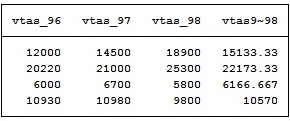
\includegraphics[height=2.7cm]{egen2.jpg}}
\end{itemize}
\end{frame}

%Cuando trabajamos con encuestas, recode resulta muchas veces un comando útil. 
%Recode permite cambiar los valores de una variable numérica según las reglas especificadas
%Si algún valor no está alcanzado por ninguna regla, se mantiene inalterado


\section{Variables de sistema}

\begin{frame}{Variables con subíndice}
\begin{itemize}
\item En STATA los comandos están \textit{vectorizados}. Esto quiere decir que cuando tipeamos
\texttt{generate x = y + z} STATA interpreta:\\
{\footnotesize
\[ x[1] = y[1] + z[1]\]
\[ x[2] = y[2] + z[2]\]
\begin{center}
...
\end{center}
\[x[\_N] = y[\_N] + z[\_N]\]}\\
\item Si en cambio escribimos \texttt{generate x = y[1]} cada observación de ``x'' será igual a la \underline{primera} observación de ``y''.  Es decir, podemos hacer referencia a observaciones específicas a través de subíndices.
\end{itemize}
\end{frame}

\begin{frame}[allowframebreaks]{Variables de sistema}
\begin{itemize}
\item Las variables de sistema \_n y \_N hacen referencia a la observación corriente y al total de observaciones, respectivamente.
\item En el marco de [by varlist:] \_n y \_N ser reinterpretan, aplicándose al interior de cada grupo definido por by varlist.
\item Supongamos que tenemos la siguiente base, que pueden descargar con: \\{\footnotesize \texttt{use http://www.stata-press.com/data/r11/gxmpl6}}\\\smallskip
\centerline{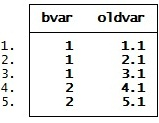
\includegraphics[height=1.8cm]{graf1.jpg}}
\item Para mostrar cómo funcionan \_n, \_N y los subíndices creamos tres variables:\\\medskip
{\footnotesize
\texttt{generate small\_n = \_n}\\
\texttt{generate big\_n = \_N}\\
\texttt{generate newvar = oldvar[1]}\\
\texttt{list}}\\\medskip
\centerline{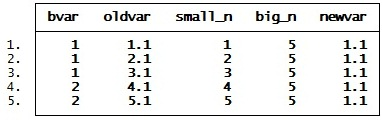
\includegraphics[height=2.2cm]{graf2.jpg}}
\item ``small\_n'' va de 1 a 5 (porque \_n va contando las obs.) y ``big\_n'' es igual a 5 (porque \_N es el total de obs.). ``newvar'' es igual al primer valor de ``oldvar''.
\item Ahora supongamos que repetimos estos pasos pero incluyendo el prefijo \texttt{by bvar:}\\\medskip
{\footnotesize
\texttt{drop small\_n big\_n newvar}\\
\texttt{bys bvar: generate small\_n = \_n}\\
\texttt{bys bvar: generate big\_n = \_N}\\
\texttt{bys bvar: generate newvar = oldvar[1]}\\
\texttt{list}}\\\medskip
\centerline{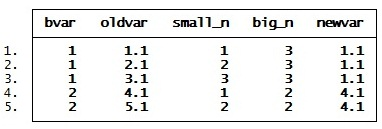
\includegraphics[height=2.2cm]{graf3.jpg}}
\item El resultado es diferente: \_n y \_N se evaluaron en relación al subconjunto definido por el by.
\end{itemize}
\end{frame}

\section{Carpetas y directorios}

\begin{frame}{Directorios}
\begin{itemize}
\item Es importante saber en qué directorio estamos parados, para abrir y guardar archivos, correr archivos .do, etc., sin necesidad de especificar un \textit{path}:
\begin{itemize}
\item \texttt{save base.dta}  \hspace{0.3 cm} $\rightarrow$ Guarda la base en la carpeta en la que estamos
\item \texttt{save ``c:\textbackslash clase1\textbackslash base.dta''}  \hspace{0.3 cm} $\rightarrow$ Guarda la base en la carpeta c:\textbackslash clase1 
\end{itemize}
\item Para saber en qué carpeta estamos usamos \texttt{pwd}
\item Para cambiar la capeta de trabajo usamos \texttt{cd}: \texttt{cd ``c:\textbackslash clase1''} nos posiciona en la carpeta c:\textbackslash clase1 
% \item Podemos crear una carpeta de trabajo desde Windows o directamente desde STATA, con \textbf{mkdir}
\item Cuando el nombre de directorios contengan espacios es obligario el uso de dobles comillas. Lo mismo sucede con los nombres de archivos.
\end{itemize}
\end{frame}

\section{Unión de bases de datos}

\begin{frame}{Unión de bases de datos}
\begin{itemize}
\item STATA permite unir bases de datos de dos maneras:
\begin{itemize}
\item Con el comando \texttt{merge} se agregan nuevas \textit{variables} a una base existente.
\item Con el comando \texttt{append} se agregan nuevas \textit{observaciones} a una base existente.
\end{itemize}
\end{itemize}
\centerline{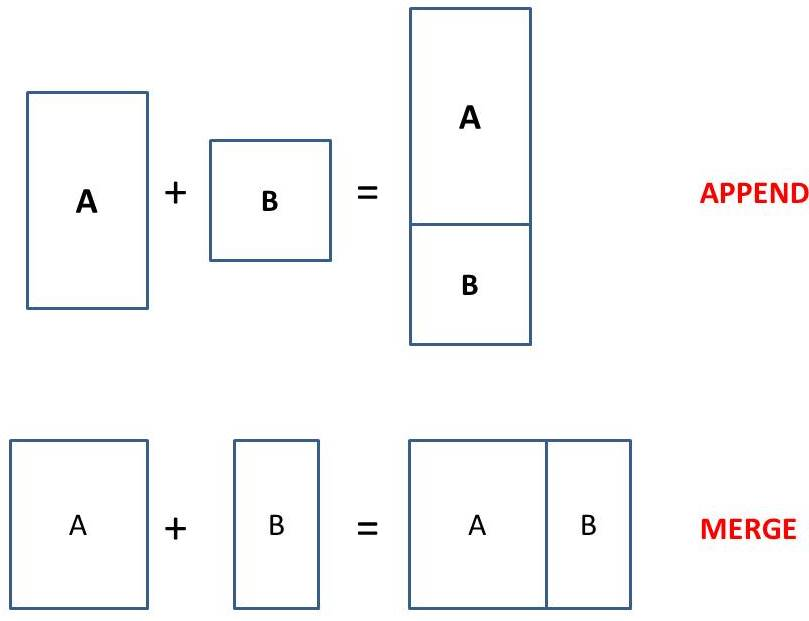
\includegraphics[height=4cm]{union.jpg}}
\end{frame}

\begin{frame}{Append}
\begin{itemize}
\item \texttt{append} añade al final de una base en memoria otra base guardada en el disco.
\item No es necesario que las bases tengan exactamente las mismas variables.
\item Si los archivos tienen variables únicas STATA resuleve esto completando con valores \textit{missing} donde es necesario
\item Supongamos que tenemos las bases ``uno.dta'' y ``dos.dta'' guardadas en el directorio donde estamos trabajando. Con los siguiente comandos creamos una única base con 5 observaciones y 3 variables:\\\smallskip
\texttt{use uno.dta, clear}\\
\texttt{append using dos}\\
\texttt{save append.dta}
\end{itemize}
\end{frame}

\begin{frame}{Append}
\begin{columns}
\begin{column}{5cm}
uno.dta\\
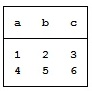
\includegraphics[height=2.5cm]{uno.jpg}\\\bigskip
dos.dta\\
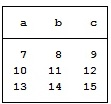
\includegraphics[height=2.5cm]{dos.jpg}
\end{column}
\begin{column}{5cm}
append.dta\\
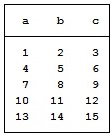
\includegraphics[height=4cm]{append.jpg}
\end{column}
\end{columns}
\end{frame}

\begin{frame}{Append}
\begin{itemize}
\item Para mostrar qué pasa si los archivos tuvieran alguna variable no comúm, cambiamos el nombre de una de las variable de la base ``dos.dta'' y guardamos los cambios: \\\smallskip
\texttt{use dos, clear}\\
\texttt{rename c d} \\
\texttt{save dos, replace}
\item Luego volvemos a hacer el \texttt{append} y observamos los nuevos resultados:\\\smallskip
\texttt{use uno, clear}\\
\texttt{apeend using dos}\\
\texttt{list}\\
\end{itemize}
\end{frame}
\begin{frame}{Append}
\begin{itemize}
\centerline{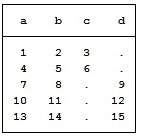
\includegraphics[height=4cm]{append2.jpg}}
\item Vemos que STATA completó con missing las observaciones para las variables no comunes.
\end{itemize}
\end{frame}

\begin{frame}{Merge}
\begin{itemize}
\item \texttt{merge} combina observaciones de la base \underline{en memoria}, llamada ``master'', con las observaciones correspondientes de la base en el \underline{disco}, llamada ``using'', a partir de una o más variables clave (identificadores).
\item Por default, después de un merge se crea una nueva variable llamada ``\_merge'' que contiene los códigos numéricos para cada observación:
\begin{itemize}
\item 1: Observación solo aparece en el ``master''
\item 2: Observación solo aparece en el ``using''
\item 3: Observación aparece en las dos
\end{itemize}
\item En el merge 1:1 una o más variables identifican de manera única a cada observación en las dos bases.
\item En el merge 1:m o m:1, varias observaciones en una base corresponden a una en la otra, o viceversa.
\end{itemize}
\end{frame}

\begin{frame}{Ejemplo merge 1:1}
\begin{itemize}
\item Supongamos que tenemos en la carpeta de trabajo las bases ``base1.dta'' y ``base2.dta'' que se presentan a continuación. 
\item En la base1 tenemos las variables edad y altura de los alumnos y en la base2, el peso. Queremos crear una única base con la información por alumno. 
\item Como tienen el mismo nivel de agregación (cada observación representa a un alumno), usamos el merge 1:1. Ingresamos los siguentes comandos:\\\smallskip
\texttt{use base1.dta, clear}\\
\texttt{merge 1:1 nombre using base2.dta}
\item Como la observación correspondiente a ``José'' estaba solo en la base2, la variable ``\_merge'' tiene valor 2.
\end{itemize}
\end{frame}

\begin{frame}{Ejemplo merge 1:1}
\begin{columns}
\begin{column}{5cm}
base1.dta\\
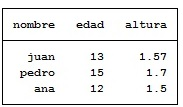
\includegraphics[height=2.5cm]{base1.jpg}\\\bigskip
base2.dta\\
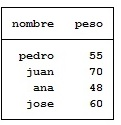
\includegraphics[height=2.5cm]{base2.jpg}
\end{column}
\begin{column}{5cm}
Resultado del merge\\
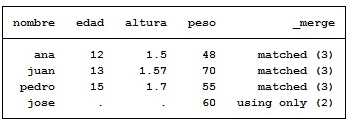
\includegraphics[height=2cm]{merge.jpg}
\end{column}
\end{columns}
\end{frame}

\begin{frame}{Ejemplo del merge m:1 y 1:m}
\begin{itemize}
\item Supongamos ahora que tenemos una base ``hogar.dta'' con características del hogar (cant. de baños y superificie) y otra base ``ind.dta'' con características de los individuos. 
\item En el primer caso la variable ``hogar'' identifica de manera única a cada observación. En el segundo caso esto no es así porque vemos que varios individuos comparten el mismo hogar: lo que identifica a cada individuo en esa base es el conjunto de variables ``hogar'' e ``ind''.
\item Para hacer el merge entre ambas bases hacemos: \\
\texttt{use hogar.dta, clear}\\
\texttt{merge 1:m hogar using ind.dta}
\item Si hubiéramos partido de la base ``ind.dta'': \\
\texttt{use ind.dta, clear}\\
\texttt{merge m:1 hogar using ind.dta}
\end{itemize}
\end{frame}

\begin{frame}{Ejemplo merge m:1 y 1:m}
\begin{columns}
\begin{column}{5cm}
hogar.dta\\
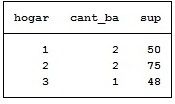
\includegraphics[height=2.5cm]{hogar.jpg}\\\bigskip
ind.dta\\
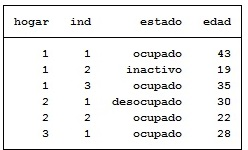
\includegraphics[height=2.5cm]{ind.jpg}
\end{column}
\begin{column}{5cm}
Resultado del merge\\
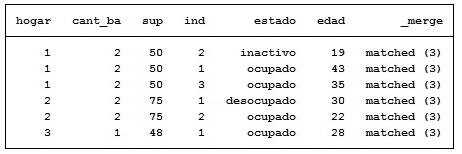
\includegraphics[height=1.9cm]{merge2.jpg}
\end{column}
\end{columns}
\end{frame}


\end{document}
\item No se afecta la precisión interna del número
\item El formato general \%9.0g es el asignado por defecto por STATA: significa que se usan hasta 9 dígitos y cero decimales
\item Si el número tiene más de 9 dígitos, STATA lo lleva a notación exponencial

